\documentclass[a4paper,
fontsize=11pt,
%headings=small,
oneside,
numbers=noperiodatend,
parskip=half-,
bibliography=totoc,
final
]{scrartcl}

\usepackage[babel]{csquotes}
\usepackage{synttree}
\usepackage{graphicx}
\setkeys{Gin}{width=.8\textwidth} %default pics size

\graphicspath{{./plots/}}
\usepackage[ngerman]{babel}
\usepackage[T1]{fontenc}
%\usepackage{amsmath}
\usepackage[utf8x]{inputenc}
\usepackage [hyphens]{url}
\usepackage{booktabs} 
\usepackage[left=2.4cm,right=2.4cm,top=2.3cm,bottom=2cm,includeheadfoot]{geometry}
\usepackage[labelformat=empty]{caption} % option 'labelformat=empty]' to surpress adding "Abbildung 1:" or "Figure 1" before each caption / use parameter '\captionsetup{labelformat=empty}' instead to change this for just one caption
\usepackage{eurosym}
\usepackage{multirow}
\usepackage[ngerman]{varioref}
\setcapindent{1em}
\renewcommand{\labelitemi}{--}
\usepackage{paralist}
\usepackage{pdfpages}
\usepackage{lscape}
\usepackage{float}
\usepackage{acronym}
\usepackage{eurosym}
\usepackage{longtable,lscape}
\usepackage{mathpazo}
\usepackage[normalem]{ulem} %emphasize weiterhin kursiv
\usepackage[flushmargin,ragged]{footmisc} % left align footnote
\usepackage{ccicons} 
\setcapindent{0pt} % no indentation in captions
\usepackage{xurl} % Breaks URLs

%%%% fancy LIBREAS URL color 
\usepackage{xcolor}
\definecolor{libreas}{RGB}{112,0,0}

\usepackage{listings}

\urlstyle{same}  % don't use monospace font for urls

\usepackage[fleqn]{amsmath}

%adjust fontsize for part

\usepackage{sectsty}
\partfont{\large}

%Das BibTeX-Zeichen mit \BibTeX setzen:
\def\symbol#1{\char #1\relax}
\def\bsl{{\tt\symbol{'134}}}
\def\BibTeX{{\rm B\kern-.05em{\sc i\kern-.025em b}\kern-.08em
    T\kern-.1667em\lower.7ex\hbox{E}\kern-.125emX}}

\usepackage{fancyhdr}
\fancyhf{}
\pagestyle{fancyplain}
\fancyhead[R]{\thepage}

% make sure bookmarks are created eventough sections are not numbered!
% uncommend if sections are numbered (bookmarks created by default)
\makeatletter
\renewcommand\@seccntformat[1]{}
\makeatother

% typo setup
\clubpenalty = 10000
\widowpenalty = 10000
\displaywidowpenalty = 10000

\usepackage{hyperxmp}
\usepackage[colorlinks, linkcolor=black,citecolor=black, urlcolor=libreas,
breaklinks= true,bookmarks=true,bookmarksopen=true]{hyperref}
\usepackage{breakurl}

%meta
%meta

\fancyhead[L]{B. Kaden \& L. Freyberg\\ %author
LIBREAS. Library Ideas, 44 (2023). % journal, issue, volume.
\href{https://doi.org/10.18452/28269}{\color{black}https://doi.org/10.18452/28269}
{}} % doi 
\fancyhead[R]{\thepage} %page number
\fancyfoot[L] {\ccLogo \ccAttribution\ \href{https://creativecommons.org/licenses/by/4.0/}{\color{black}Creative Commons BY 4.0}}  %licence
\fancyfoot[R] {ISSN: 1860-7950}

\title{\LARGE{Makerspaces und Library Labs in wissenschaftlichen Bibliotheken -- zwischen physischem Raum und forschungsorientierter Ausrichtung}}% title
\author{Ben Kaden und Linda Freyberg} % author

\setcounter{page}{1}

\hypersetup{%
      pdftitle={Makerspaces und Library Labs in wissenschaftlichen Bibliotheken -- zwischen physischem Raum und forschungsorientierter Ausrichtung},
     pdfauthor={Ben Kaden, Linda Freyberg},
      pdfcopyright={CC BY 4.0 International},
      pdfsubject={LIBREAS. Library Ideas, 44 (2023).},
      pdfkeywords={Digital Makerspaces, Library Labs, Kompetenzvermittlung, Co-Creation, wissenschaftliche Bibliotheken, Scholarly Makerspaces},
      pdflicenseurl={https://creativecommons.org/licenses/by/4.0/},
      pdfurl={https://doi.org/10.18452/28269},
      pdfdoi={10.18452/28269},
      pdflang={de},
      pdfmetalang={de}
     }



\date{}
\begin{document}

\maketitle
\thispagestyle{fancyplain} 

%abstracts
\begin{abstract}
\noindent
In den 2010er Jahren begann die Diskussion über Makerspaces in
Bibliotheken als Reaktion auf die Digitalisierung und den Wunsch nach
neuen Nutzungsmöglichkeiten. Diese Räume erweiterten Bibliotheken zu
kollaborativen Zentren für digitales Gestalten und gemeinsame
Tool-Anwendung. Sie fördern dabei kreative Zusammenarbeit und
Kompetenzvermittlung in Hinblick auf digitale Verfahren. Der vorliegende
Text ist als Vorlage für die weitere Beschäftigung mit Makerspaces und
Library Labs in wissenschaftlichen Bibliotheken gedacht. Dafür
betrachtet er Beispiele aus wissenschaftlichen Bibliotheken und
diskutiert Ziele, Konzepte sowie Ausstattungsanforderungen. Diese werden
in einer Übersicht zu Konzeptmerkmalen sowie einer Makerspace-Matrix
zusammengefasst. Es wird deutlich, dass Digital Makerspaces und Library
Labs agile Innovationsorte sind, die über unterschiedliche Formate und
Methoden wie Co-Creating und Peer-to-Peer-Lernen interdisziplinäre
Zusammenarbeit und inklusives Lernen fördern.

\begin{center}\rule{0.5\linewidth}{0.5pt}\end{center}

In the 2010s, the discussion about makerspaces in libraries began as a
reaction to digitalisation and the desire for new ways of use. These
spaces expanded libraries into collaborative centres for digital
creation and joint tool use. They encourage creative collaboration and
skills transfer with regard to digital processes. This text is intended
as a starting point for further exploration of makerspaces and library
labs in academic libraries. To this end, it examines examples from
academic libraries and discusses objectives, concepts as well as
equipment requirements. These are summarised in an overview of concept
features and a makerspace matrix. It emerges that digital makerspaces
and library labs are agile places of innovation that promote
interdisciplinary collaboration and inclusive learning through different
formats and methods such as co-creation and peer-to-peer learning.
\end{abstract}

%body
\hypertarget{makerspaces-in-bibliotheken}{%
\section{Makerspaces in
Bibliotheken}\label{makerspaces-in-bibliotheken}}

Seit den frühen 2010er Jahren wird die Zusammenführung von Ideen des
\enquote{Making} mit Bibliotheken diskutiert.\footnote{Colegrove, 2013;
  Dougherty, 2013} Teilweise resultierte dies aus der Beobachtung
beziehungsweise der Erwartung, dass durch die zunehmende Digitalisierung
von Beständen und vor allem auch durch die Auflösung analoger
Nachweissysteme wie Zettelkataloge Raum in Bibliotheken für neue
Nutzungsformen verfügbar wird.\footnote{Colegrove, 2013; Bonte, 2021}
Dazu wurde eine Erwartung an die Bibliotheken spürbar, das Erlebnis der
Institution durch die Besuchenden und Nutzenden stärker aufzugreifen und
mit einer möglichst hohen Aufenthalts- und Erlebensqualität zu
unterlegen.\footnote{Bonte, 2021} Die Bibliothek als \enquote{dritter
Ort}, Cafés und Begegnungszonen in Bibliotheken bildeten vor allem in
Öffentlichen Bibliotheken einen Ansatz. Makerspaces repräsentierten
einen anderen.

Letztere wurden durch die Herausbildung von gemeinsam genutzten und
räumlich fixierten Angeboten digitaler Werkzeuge für eine allgemeine
Nutzung, also hier: Makerspaces, sowie die Praxis des \enquote{digital
making} und einer sich entfaltenden Makerbewegung begleitet.\footnote{siehe
  exemplarisch für ein Angebot in Barcelona Diaz, Tomàs, Lefebvre, 2021}
Deren Ort war zunächst nicht einmal unbedingt in Bibliotheken.

Die Bibliotheken kamen als Orte der Vermittlung von digitalen
Kompetenzen und zugleich mit dem Anspruch eines \enquote{digitalen
Empowerment} und einer Digitalisierung ins Spiel.\footnote{Smolarczyk,
  Kröner (2023); Colegrove, 2013} Dabei entfaltete sich ein Verständnis
der Bibliotheksnutzung jenseits der Medienrezeption, das mit der bereits
existierenden Makerbewegung korrelierte und unter \enquote{making rather
than merely consuming}\footnote{Colegrove, 2013, S. 3} gefasst wurde.

Die Neuigkeit dieser schöpferischen Tätigkeit in Bibliotheken lag in der
Kollaborativität und in der Erweiterung auf Nutzungsformen jenseits der
Textrezeption und -produktion. Für diese Praxis lassen sich drei
Konzeptlinien unterscheiden: Während, erstens, \enquote{Co-Working} die
Zusammenarbeit zwischen Nutzenden betont, stehen, zweitens,
\enquote{hackerspaces}\footnote{Schrock, 2014} vor allem für die
digitale Komponente und, drittens, \enquote{fab(rication) labs} für die
Nutzung digitaler Werkzeuge bei der Ideenfindung.\footnote{Colegrove,
  2013} Die Konzepte müssen dabei aber nicht getrennt betrachtet werden,
sondern können auch kombiniert, zum Beispiel als digitaler
\enquote{Makerspace}, angeboten werden.\footnote{Ebenda}

Das Ziel dieser Makerspaces war allerdings keine festgelegte
Fokussierung auf bestimmte Nutzungsresultate. Vielmehr sollten sie
prinzipiell und ergebnisoffen die Anregung zu einer vertiefenden und
multiperspektivischen Auseinandersetzung und eine domänenübergreifende
Kompetenzvermittlung unterstützen.\footnote{Ebenda} Eine spezialisierte
technische Perspektive war ausdrücklich nicht vorgesehen.\footnote{Martinez,
  Stager, 2019} Wissen sollte bevorzugt in Form eines Co-Creatings und
auf Peer-to-Peer-Ebene vermittelt werden.\footnote{Mersand, 2021}
Anschlüsse zur vorberuflichen Bildung waren ebenfalls
denkbar.\footnote{Wand, Tiepmar, 2023} All diese Prozesse sollten in
einem informellen und zugleich motivierenden Setting
erfolgen.\footnote{Smolarczyk, Kröner, 2023; Julian, Parrott, 2017:
  \enquote{The purpose of the makerspace is to create a comfortable
  environment for users to experiment, create and learn within a
  controlled setting.}}

Die dafür erforderlichen Rahmenbedingungen fanden sich traditionell
stärker in Öffentlichen Bibliotheken durch ihre Ausrichtung auf
Weiterbildung und Freizeitgestaltung. So überrascht es nicht, dass der
erste Makerspace in einer deutschen Bibliothek 2013 in der
Stadtbibliothek Köln eröffnet wurde.\footnote{Vogt, Scheurer, Pohla,
  2016} Es folgten zahlreiche Makerspaces, unter anderem an zwei
Standorten in Berlin-Mitte (FreeLab -- Makerspace in der
Schiller-Bibliothek\footnote{\url{https://www.berlin.de/stadtbibliothek-mitte/angebote/makerspace/schiller-bibliothek-mit-hugo-jugendmedienetage/freelab-makerspace-in-der-schiller-bibliothek-oeffnet-sich-fuer-die-community-845942.php}}
und in der Bezirkszentralbibliothek Philipp Schaeffer\footnote{\url{https://www.berlin.de/stadtbibliothek-mitte/bibliotheken/bezirkszentralbibliothek-philipp-schaeffer/aktuelle-projekte/}}).
Ein weiteres Beispiel ist das im Jahr 2017 eröffnete LibraryLab der
Zentralbibliothek der Stadtbüchereien Düsseldorf.\footnote{\url{https://www.duesseldorf.de/stadtbuechereien/bibliotheken/librarylab}}

Das Angebotsspektrum dieser Einrichtungen reicht von
Digitalisierungstechnik und digitalen Bearbeitungswerkzeugen für
Fotografien, analogen Medienträgern sowie 3D-Objekten über die Ausleihe
von Näh- und Stickmaschinen bis zum Erproben von 3D-Druckern,
VR-Brillen, Spielekonsolen und Robotern beziehungsweise
Robotik-Programmier-Sets. Mit diesen Angeboten übernahmen Öffentliche
Bibliotheken eine Vorreiterrolle für aktivierende und
kompetenzvermittelnde Nutzungsformen. Dies führte zu wichtigen Impulsen
auch für wissenschaftliche Einrichtungen, erzeugte aber auch bestimmte
Vorstellungsbilder und Erwartungshaltungen für das Konzept
\enquote{Makerspace}, die sich nicht mit den Zielen für
wissenschaftliche Einrichtungen decken.

\hypertarget{makerspaces-in-wissenschaftlichen-bibliotheken}{%
\section{Makerspaces in wissenschaftlichen
Bibliotheken}\label{makerspaces-in-wissenschaftlichen-bibliotheken}}

In der Auseinandersetzung mit dieser Herausforderung soll es in diesem
Beitrag um eine Einordnung des Konzepts und den Vorschlag einer
Anwendungsperspektive für Makerspaces in wissenschaftlichen
Bibliothekskontexten gehen. Die Schwerpunkte liegen erwartungsgemäß
abstrakt auf der digital forschenden Arbeit und einer Auseinandersetzung
mit digitalen und digitalisierten Beständen.

\hypertarget{zielstellung-produkt-oder-kompetenz}{%
\subsection{Zielstellung: Produkt oder
Kompetenz?}\label{zielstellung-produkt-oder-kompetenz}}

Für Makerspaces in wissenschaftlichen Bibliotheken wurde lange
diskutiert, inwieweit Makerspaces ein genuin neues Konzept oder die
Fortsetzung der genannten bereits bestehenden Angebote öffentlicher
Bibliotheken sind.\footnote{Willett, 2016} Für ihre Zielstellung zeigten
sich zwei Pole: erstens die Produktorientierung und zweitens die
Lernorientierung.\footnote{Willett, 2016} Dies spiegelt sich in der
Perspektive der internationalen Library Labs-Bewegung auf den (offenen)
Umgang mit Forschungs- und Kulturdaten.\footnote{Eine Liste der
  vorwiegend angloamerikanischen Library Labs findet sich hier:
  \url{https://www.rss4lib.com/library-labs/}} Die im Jahr 2018 von der
British Library gestartete \#buildinglibrarylabs-Initiative konzentriert
sich auf offene Schnittstellen für Kulturdaten, die eine kreative und
wissenschaftliche Weiterverwendung ermöglichen sowie die
Weiterentwicklung von Services und die Weiterbildung des
Personals.\footnote{Siehe Neudecker, 2018}

\begin{figure}
\centering
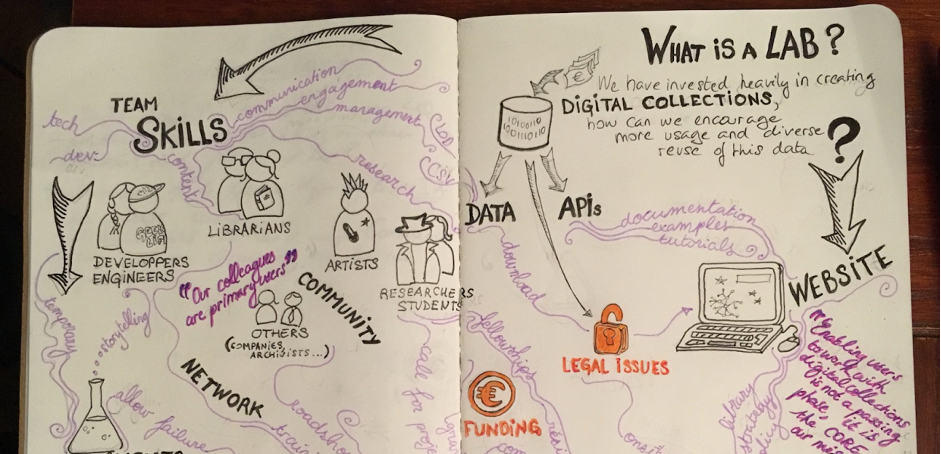
\includegraphics{abbildung_1.png}
\caption{\#buildlibrarylabs sketchnotes. Bildnachweis: Creator:
Emmanuelle Bermes, Date: September 2018 Institution: Bibliotheque
national de France, {[}CC-BY{]}}
\end{figure}

Weitere konzeptionelle Entwicklungslinien lassen sich auch aus dem
Kontext von \enquote{Fab Labs} ermitteln.\footnote{Brandenburger et al.,
  2023, S. 147f.} So gibt es zunächst unterschiedliche Bildungskonzepte:
Die ergebnisoffene selbstorganisierte, oft Peer-to-Peer-orientierte
Ausrichtung von Labs oder Makerspaces trifft auf Curricula und linear
ausgerichtete Vorstellungen des Lernens. Weiterhin besteht eine Spannung
zwischen den spezifischen Nutzungskompetenzen und handwerklichen
Methoden auf der einen Seite und den abstrahierbaren, sozialen und
individuellen Erfahrungen wie Lernkompetenz allgemein sowie der
Selbstwirksamkeit der Nutzenden auf der anderen Seite.

Generell ist eine Doppelrolle von Makerspaces und Labs zu beobachten:
Sie vermitteln konkrete Kompetenzen und Zugänge und fungieren zugleich
als Orte des (pluriversellen) Co-Creating\footnote{Ferrari, 2022} und
wirken damit im Sinne einer sozialen Innovation.\footnote{Zum Konzept
  von \enquote{Social Innovation} siehe McGowan, Westley, 2015}

\hypertarget{erwartungen-und-ausrichtungen}{%
\subsection{Erwartungen und
Ausrichtungen}\label{erwartungen-und-ausrichtungen}}

Daraus ergeben sich unterschiedliche Erwartungshaltungen. So werden
Digital Makerspaces und Scholarly Makerspaces sowie Labs in
wissenschaftlichen Zusammenhängen häufig direkt mit Digital Humanities
assoziiert. Entsprechend erfolgt eine Konzeptentwicklung meist
unmittelbar mit dieser Ausrichtung, mitunter mit dem ausdrücklichen
Anspruch der Entwicklung einer \enquote{Laborkultur der digitalen
Geisteswissenschaften}.\footnote{Mischke, 2023 {[}ohne Seitenzahl{]}}
Diese Spezialisierung ergibt in bestimmten Zusammenhängen Sinn. In
anderen verengt sie jedoch die Perspektive und führt zur Exkludierung
bestimmter Zielgruppen.

In der Umsetzung zeigt sich bisher keine einheitliche Linie der
Angebote, sondern ein durch paralleles konzeptionelles
\enquote{Erfinden} geprägtes Entwickeln, das jeweils von Anforderungen
und Rahmenbedingungen der konkreten Institution geprägt wird.

\hypertarget{hardware}{%
\section{Hardware}\label{hardware}}

Entsprechend variiert auch die Ausgestaltung und Hardwareausstattung der
Labs/Makerspaces. In vielen Fällen wird auch für wissenschaftliche
Zusammenhänge eine Schwerpunktsetzung auf physische Werkzeuge
(\enquote{3D printing, laser cutting, and electronics}\footnote{Radniecki,
  Klenke, 2017, S. 16}) als Angebot, mit einem deutlichen Schwerpunkt
auf 3D-Druck, verfolgt.\footnote{Ebenda} Der Anschluss an die
traditionelle Makerbewegung liegt dabei offen zutage.

Daraus ergibt sich eine weitere Notwendigkeit der diskursiven
Differenzierung in auf Hardware orientierten Vermittlungs- und
Nutzungskonzepten, oft im Zusammenhang mit technischen Wissenschaften,
und bestands- und sammlungszentrierte Ansätzen vor allem für die
Geistes- und Kulturwissenschaften sowie die Digital Humanities.

Im ersten, technischeren Diskurs werden erwartbar übergreifend
inhaltliche Schwerpunkte des technischen Machens, oft auch Prototyping,
mit Anschluss entweder an die Informatik oder an STEM (science,
technology, engineering and math) betont.\footnote{Ebenda; Julian,
  Parrott, 2017} In der Umsetzung stehen Bibliotheken allerdings dabei
häufig in Konkurrenz zu jeweils spezialisierten Forschungslabs in
Fakultäten, Instituten und Fachbereichen, die entsprechende Angebote
sowohl für die Forschung als auch für die Methodenvermittlung
einsetzen.\footnote{So betreibt das Institut für Bibliotheks- und
  Informationswissenschaft der Humboldt-Universität zu Berlin einen so
  genannten \enquote{Flexpool}, der gezielt Kollaboration und die
  Auseinandersetzung mit digitalen Technologien auch auf der
  Hardwareebene unterstützt.} Für Bibliotheken bleibt in solchen
Gemengelagen möglicherweise die Rolle der Ergänzung als ein einerseits
allgemeiner ausgerichtetes Angebot und andererseits eines noch
offeneren, weil nicht unmittelbar durch fachkulturelle Anforderungen und
Ziel begrenztes Übungsfelds.

\hypertarget{makerspaces-als-kuxfcche}{%
\section{\texorpdfstring{Makerspaces als
\enquote{Küche}}{Makerspaces als ``Küche''}}\label{makerspaces-als-kuxfcche}}

Entscheidend ist in allen Szenarien die Aktivierung der Nutzenden, wofür
der ehemalige stellvertretende Generaldirektor der Staats-, Landes- und
Universitätsbibliothek (SLUB) Dresden, Achim Bonte, das Bild einer
\enquote{Küche} im Gegensatz zum \enquote{Lebensmittelladen}
fand.\footnote{Siehe Bonte, 2021}

So findet sich an der SLUB Dresden auch ein viel zitiertes
Musterbeispiel für einen derart ausgerichteten Makerspace, der in diesem
Fall in Kooperation mit der Technischen Universität Dresden
entstand.\footnote{Siehe
  \url{https://www.slub-dresden.de/mitmachen/slub-makerspace}}

\begin{figure}
\centering
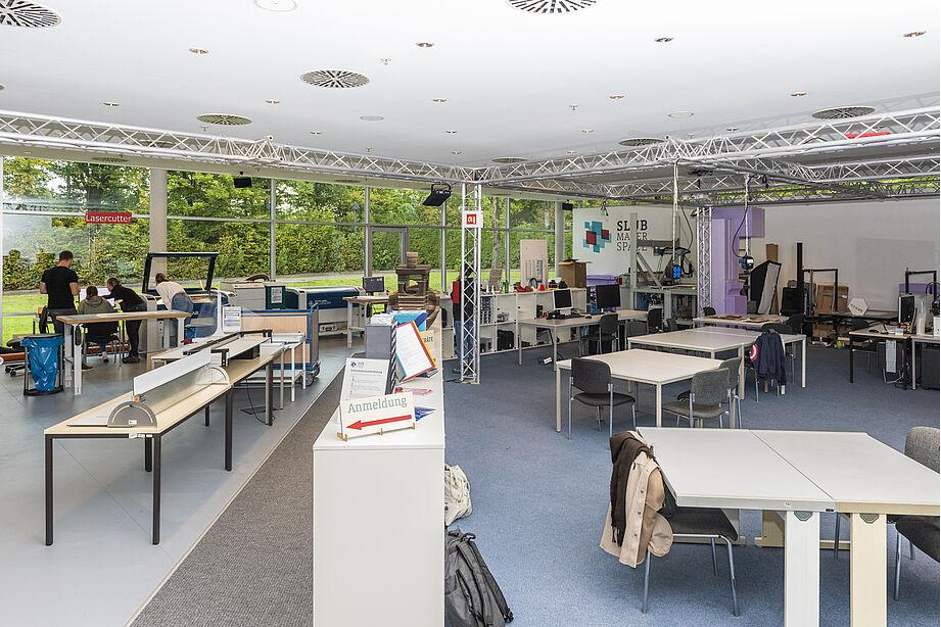
\includegraphics{abbildung_2.png}
\caption{Werkstatt SLUB Dresden Makerspace. Bildnachweis:
\url{https://www.slub-dresden.de/mitmachen/slub-makerspace/arbeitsraeume}}
\end{figure}

Neben dem großen Werkstattraum (siehe Abbildung 1) bietet dieser
Makerspace Arbeitsplätze, ein Fotostudio sowie Veranstaltungs- und
Besprechungsräume. Die Ausstattung beinhaltet unter anderem Werkzeuge,
eine Lötstation, 3D-Drucker (für Filament und Gips), 3D-Scanner und
3D-Drucker. In Angebot und Programm orientiert sich der Makerspace an
den Curricula technischer Studiengänge wie Maschinenbau und legt einen
starken Fokus auf die Bereitstellung von Hardware.\footnote{Wand,
  Tiepmar, 2023}

Hinter einem weiteren 2015 erstmals als \enquote{Laboratory}
eingerichteten Angebot steht dagegen die Vorstellung, dass das Wissen in
der Gegenwart nicht mehr auf Text und Datenbestände klassischen
Zuschnitts reduziert betrachtet und vermittelt werden kann, sondern auch
stark Technologie geprägte, nicht textuelle Wissenssysteme und -kulturen
relevant werden.\footnote{Bonte, 2021} Ein \enquote{SLUB-Textlab}
ergänzt dieses als \enquote{offene Werkstatt für sämtliche Arbeiten an
Texten} beziehungsweise einen \enquote{Makerspace der Worte}.\footnote{\url{https://www.slub-dresden.de/mitmachen/slub-textlab}}

\hypertarget{anwendungsfuxe4lle}{%
\section{Anwendungsfälle}\label{anwendungsfuxe4lle}}

Anhand von drei Anwendungsfällen soll nachfolgend die Bandbreite der
Anforderungen an Scholarly Makerspaces und Digital Makerspaces
illustriert werden. Die beiden Autor*innen des Beitrags waren bzw. sind
in die Entwicklung dieser Angebote eingebunden.\footnote{Ben Kaden in
  den Scholarly Makerspace der Humboldt-Universität (Projektstudie) und
  den Digital Makerspace an der Klassik Stiftung Weimar
  (Konzeptentwicklung) und Linda Freyberg ist eine der
  wissenschaftlichen Koordinator*innen des Digital History of Education
  Lab (DHELab) der BBF des DIPF.}

\hypertarget{scholarly-makerspace-der-ub-der-hu-berlin}{%
\subsection{Scholarly Makerspace der UB der HU
Berlin}\label{scholarly-makerspace-der-ub-der-hu-berlin}}

Der Scholarly Makerspace an der Universitätsbibliothek der
Humboldt-Universität zu Berlin lässt sich in ein generelles
Innovationsbemühen des damaligen Bibliotheksdirektors Andreas Degkwitz
einordnen. Die Konzeptentwicklung folgte dem anhaltenden Trend,
Bibliotheken offensiv als aktive Forschungsinfrastrukturen
aufzustellen.\footnote{Vergleiche dazu auch Mischke, 2023} Dieser zeigte
sich in mehreren Projekten und Projektanträgen zur
bibliothekswissenschaftlichen Auseinandersetzung mit sich entwickelnden
Anforderungen an Bibltiotheksdienstleistungen durch digital geprägte
Forschung.\footnote{Siehe, unter anderem, Kleineberg, Kaden, 2017} Die
Idee der Einrichtung eines, so der Arbeitstitel, \enquote{Scholarly
Makerspace} an der Universitätsbibliothek entwickelte sich aus diesem
Kontext. Für die Umsetzung wurden zunächst für die Durchführung einer
Projektstudie an der Humboldt-Universität zu Berlin bei der DFG Mittel
beantragt.\footnote{Kaden, Kleineberg, 2019}

Ein Teil der Idee war, Universitätsbibliotheken forschungsnäher an
Entwicklungen in den Digital Humanities und digital geprägten
Geisteswissenschaften heranzuführen. Ein zweiter Aspekt lag in der
Überlegung, den Bestand von Bibliotheken erweitert zu denken und auch
Forschungsobjekte beziehungsweise -datensätze zur Verfügung zu stellen
sowie die für die Erforschung notwendigen digitalen Werkzeuge und
entsprechende Nutzungskompetenzen zu vermitteln.\footnote{Ebenda}

Im Folgeantrag zur eigentlichen Einrichtung eines solchen
\emph{Scholarly Makerspace} als Proof-of-Concept wurde entsprechend der
Ausdruck \enquote{Tool Literacy} im Sinne der Befähigung zur Nutzung
digitaler Forschungswerkzeuge in den Mittelpunkt gerückt. Ein weiterer
Innovationspunkt lag in der vorgesehenen konkreten Beratung und
gegebenenfalls Begleitung von antragstellenden Personen bei der Auswahl
passender und möglicherweise durch die Universitätsbibliothek
bereitstellbarer Werkzeuge und Inhalte.

Die Konzeptstudie differenzierte über Interviews und eine Bedarfsanalyse
Potentiale und umsetzungsrelevante Aspekte für \enquote{Scholarly
Makerspaces} und bildete die Grundlage für das von DFG geförderte
Projekt zur prototypischen Implementierung eines Scholarly Makerspaces
an der Universitätsbibliothek der Humboldt-Universität zu
Berlin.\footnote{Degkwitz, 2020; Degkwitz, 2021}

Die eigentliche Umsetzung des Prototypen erfolgt seit Frühjahr
2022.\footnote{Grallert, 2022} Erwartungsgemäß erfolgten Anpassungen
sowohl konzeptionell als auch im Umsetzungsprogramm. Durch die
Kooperation mit dem Lehrstuhl für Digital History an der
Humboldt-Universität ergab sich eine noch stärkere Einbindung in die
Digital-Humanities-Aktivitäten an der Universität.

Dies schlägt sich auch in der Definition der Zielgruppen nieder: Der
Scholarly Makerspace ist laut aktueller Selbstbeschreibung ein
\enquote{Lernort für digitale Werkzeugkompetenz in den Geistes- und
Kulturwissenschaften}.\footnote{\url{https://makerspace.hypotheses.org/}}
Die Zielgruppen

\begin{quote}
\enquote{sind Lehrende und Forschende der Humboldt-Universität in allen
Phasen ihrer wissenschaftlichen Karrieren. Erstere sollen durch den
Ansatz von train-the-trainer in der Vermittlung von Digital Humanities
in der Lehre, letztere im gesamten Prozess von der Konzeption eines
Forschungsprojektes bis zur Umsetzung unterstützt werden.}\footnote{Grallert,
  2022}
\end{quote}

Das Tool- und Kompetenzvermittlungsangebot ist aktuell auf Methoden,
Konzeptverständnis und Programmiersprachen ausgerichtet.\footnote{\url{https://makerspace.hypotheses.org/das-werkzeugregal}}
Die aktuelle räumliche Integration in das
Jacob-und-Wilhelm-Grimm-Zentrum erfolgt bisher vor allem als Projektbüro
und Beratungsraum. Viele Veranstaltungen finden digital statt. Für
andere werden vorhandene Räumlichkeiten im Gebäude oder der
Humboldt-Universität temporär genutzt.

\hypertarget{digital-makerspace-an-der-haab-der-ksw-weimar}{%
\subsection{Digital Makerspace an der HAAB der KSW
Weimar}\label{digital-makerspace-an-der-haab-der-ksw-weimar}}

An der Herzogin Anna Amalia Bibliothek (HAAB) der Klassik Stiftung
Weimar wird im Rahmen des Forschungsverbunds Marbach Weimar Wolfenbüttel
seit Mai 2022, aufbauend auf Vorarbeiten der Stiftung, ein Digital
Makerspace entwickelt. Die Anforderungen unterscheiden sich aus drei
Gründen erheblich von Makerspaces in Universitätsbibliotheken: Erstens
steht diesem Fall weniger ein Bezug zur akademischen Lehre und Forschung
im Mittelpunkt. Zweitens ist der inhaltliche Bezugsrahmen durch
außerordentlich umfangreiche und einzigartige Sammlungsstrukturen
geprägt. Drittens hält die Klassik Stiftung Weimar bereits diverse
öffentlichkeitsbezogene Angebote auch digitaler Art vor.\footnote{Kaden,
  2022a}

Das aus dem Forschungsverbund MWW finanzierte Projekt zum Digital
Makerspace hat das Ziel, ein möglichst fortgeschrittenes und
implementierungsreifes Konzept vorzulegen und geeignete Formatansätze
unter anderem über prototypische Veranstaltungen zu
entwickeln.\footnote{Kaden, 2022b}

Aus den Vorarbeiten an der Klassik-Stiftung ergab sich zunächst
ebenfalls eine Orientierung auf die Digital Humanities, was, so eine
Annahme, mit einer Kooperationsperspektive zum entsprechenden
Schwerpunkt an der Bauhaus Universität Weimar korrelieren könnte.
Allerdings scheint die Perspektive des Forschungsfeldes im dortigen
Fachbereich Medien nicht dauerhaft konsolidiert, weshalb diese
Entwicklung nicht vorrangig verfolgt wurde.

Zugleich bieten sowohl die Sammlungen und die Programmarbeit der Klassik
Stiftung als auch die Breite der Forschungsthemen vor allem im
Fachbereich Medienwissenschaft an der Bauhaus Universität andere
potentielle Kooperationsbereiche, die eine breitere Perspektive
nahelegen. Die Digital Humanities werden nach aktuellem Stand als
optionale Entwicklungslinie im entstehenden Konzept empfohlen. Der
Schwerpunkt liegt nun jedoch auf den Sammlungen und damit auf der
digitalen Sammlungsaktivierung, -erfahrung, -bearbeitung und
-beforschung sowie -vermittlung, also des \enquote{Making}\footnote{Kaden,
  2023a} einerseits und der so genannten \enquote{digitalen
Sammlungsforschung} beziehungsweise sogar \enquote{digitalen
Sammlungsvermittlungsforschung} als Metafokus andererseits.\footnote{Kaden,
  Köhler, 2023}

Die Zielgruppenausrichtung ist zweigeteilt. Für die Sammlungsforschung
wird sie auf professionelle Kultur- und Forschungscommunities bezogen,
bei der allgemeinen Vermittlung in Übereinstimmung mit dem Leitbild der
Klassik Stiftung breiter gesellschaftlich ausgerichtet und damit
inklusiver gefasst. Umfassende Bestände an bereits digitalisierten
Sammlungsgütern bieten eine umfassende Materialgrundlage, die für beide
Ausrichtungen aktivierbar ist.

Der Digital Makerspace selbst wird nach dem entstehenden Konzept als
Facilitator und offener Raum beziehungsweise \enquote{Möglichkeits- und
Ermöglichungsraum}\footnote{Kaden, 2022b} verstanden, der anhand der
Schlagworte Inspiration - Exploration - Kommunikation\footnote{Kaden,
  2022b} vor allem methodische Unterstützung und Begleitung für die
nutzenden Communitys bietet.

Inhaltlich sollen als eine dritte Zielgruppe die Abteilungen der Klassik
Stiftung motiviert werden, sich, zum Beispiel über Ideathons\footnote{Köhler,
  2023}, kollaborativ zu digitalen Entwicklungsmöglichkeiten
auszutauschen. Die Besonderheit dieses Makerspaces ist also auch eine
Wirkung als Innovationsplattform für die Einrichtung selbst. So kann der
Digital Makerspace eigene Experimentier- und Interaktionsmöglichkeiten
für die jeweiligen Themenjahre und als Ausstellungsbegleitung
anbieten.\footnote{ebenda}

Geplant ist zudem, über den Virtuellen Forschungsraum\footnote{\url{https://www.mww-forschung.de/en/home}}
des Forschungsverbunds MWW einen virtuellen \enquote{Digital Makerspace}
als ortsunabhängiges Ergänzungsangebot für die Interaktion mit
Sammlungsobjekten und die Präsentation der Aktivitäten des Digital
Makerspace weiterzuführen. Dies scheint insofern für die Klassik
Stiftung besonders naheliegend, da sie viele externe Zielgruppen
anspricht. Eine andere lokale virtuelle Plattform ist die
\enquote{Weimar+ App}. \footnote{\url{https://www.klassik-stiftung.de/en/digital/app/}}
Deren Integration mit dem Digital Makerspace ist eine weitere
Entwicklungsrichtung, die sich besonders für topologisch ausgerichtete
Projekte anbietet.

Der konkrete Raum vor Ort im Studienzentrum der Herzogin Anna Amalia
Bibliothek soll in einen Arbeitsbereich mit Workstations, einen
Begegnungs- und Kommunikationsbereich und einen Präsentationsbereich
differenziert werden. Aus baulichen Gründen werden Arbeits- und
Kommunikationsbereich in einem Raum gebündelt, weshalb die funktionale
Unterscheidung über die Programmgestaltung und Nutzungszeiten abgebildet
werden muss.

\hypertarget{digital-history-of-education-lab-dhelab-der-bbf-des-dipf}{%
\subsection{Digital History of Education Lab (DHELab) der BBF des
DIPF}\label{digital-history-of-education-lab-dhelab-der-bbf-des-dipf}}

Das DHELab der BBF \textbar{} Bibliothek für Bildungsgeschichtliche
Forschung des DIPF \textbar{} Leibniz-Institut für Bildungsforschung und
Bildungsinformation in Berlin wurde im Herbst 2023 neu gegründet und
soll zukünftig "ein physischer und virtueller Ort werden, an dem mit
Beständen innovativ gearbeitet, Methoden und Tools für die digitale
Bildungsgeschichte erprobt, vermittelt und präsentiert werden."
\footnote{\url{https://bbf.dipf.de/de/arbeiten-lernen/dhelab}} Die
Gründung des Labs ist ein Teil der Strategie der "digitalen BBF", die
auf die digitale Transformation der Geisteswissenschaften (Digital
Humanities), insbesondere der Historischen Bildungsforschung, Bezug
nimmt. Diese beinhaltet nicht nur das Arbeiten mit digitalen Quellen und
die Befähigung, neue Tools und Methoden anzuwenden, sondern auch deren
Funktionsweisen zu verstehen und kritisch zu reflektieren.

Generell soll das DHELab an der Schnittstelle zwischen Forschung und
Informationsinfrastruktur angesiedelt sein.

"In der BBF arbeiten Forscher*innen der Bildungsgeschichte,
Bibliothekar*innen, Archivar*innen, Informationswissenschaftler*innen
und IT-Entwickler*innen zusammen. Sie bringen ihren Erfahrungsschatz und
ihre Kenntnisse, über die sie in den Bereichen Forschung mit
computationalen Methoden, Erzeugung, Bereitstellung und Archivierung
sowie Analyse, Präsentation und digitale Publikation von Forschungsdaten
verfügen, in das DHELab ein." \footnote{Ebenda}

In Anlehnung an die Idee der FabLabs und Makerspaces will das DHELab
Forschende befähigen, selbst aktiv zu werden. Strategisch möchte das
DHELab die Möglichkeiten des kollaborativen Arbeitens und der Vernetzung
mit Blick auf die zunehmend interdisziplinären Anforderungen an
Forschungsprojekte erweitern und neue Kooperationen gezielt fördern.

Die Zielgruppe des DHELab umfasst daher prinzipiell alle zur
Bildungsgeschichte forschenden und daran interessierten Menschen.
Darüber hinaus sollen mit dem Angebot die Communities der Digital
Humanities, insbesondere der Digital History, erreicht
werden.\footnote{Ebenda}

Das DHELab bietet zunächst Vorträge und Workshops an. Darüber hinaus
entwickelt es gemeinsam mit den Fachcommunitys weitere bedarfsgerechte
Angebote. Dabei ist das DHELab offen für neue Ideen, Formate und
Inhalte, die auch von den Nutzenden selbst eingebracht werden sollen .

Im September 2023 startete das Lab mit einem Soft-Launch, bei dem das
Konzept vorgestellt wurde. Für eine übergeordnete fachwissenschaftliche
Einordnung sorgten eine Keynote zu Methoden und Tools in der Digital
History von Torsten Hiltmann sowie ein Input zum Potential von 3D-Daten
für die bildungshistorische Forschung und der Möglichkeit, vor Ort mit
einem 3D-Handscanner Objekte zu erfassen.

Ab Oktober 2023 ist das Lab mit einem monatlichen Online-Vortrags-Format
"Last Friday's Lab Talk" zu Themen wie Visualisierung, kritische
Quellenkritik und Text Mining gestartet.\footnote{Veranstaltungen siehe
  ebenda sowie Mailingliste:
  \url{https://www.listserv.dfn.de/sympa/info/dhelab}.}

Ab 2024 wird das Angebot um (vor Ort-)Workshops zu Themen wie
Transkription und Erschließung und Aufbereitung historischer Bestände
zum Beispiel mit TEI\footnote{\url{https://tei-c.org/}} erweitert .

Vor Ort präsentiert sich das DHELab bislang als leerer Raum. Dies stellt
gemäß des aktuellen Entwicklungsstandes eine bewusste Entscheidung dar,
da die Raumausstattung sich strikt an den Bedürfnissen der Forschenden
orientieren soll.

Diese Kompetenzorientierung geht mit einer für die Forschung wichtigen
Befähigung zur kritischen Reflexion der angewandten Verfahren und
Quellen einher. Zu diesem Zweck wird im Jahr 2024 eine umfassende
Erhebung innerhalb der bildungshistorischen Community durchgeführt, die
einerseits den Status Quo im Umgang mit historischen Quellen, digitalen
Tools und Methoden sowie zukünftige Forschungsszenarien ermitteln soll.
Basierend auf den Ergebnissen dieser Studie sowie der Berücksichtigung
bibliotheks- und informationswissenschaftlicher Forschung sowie der
digitalen Geisteswissenschaften zu Makerspaces und Library Labs, soll
der Raum peu a peu gestaltet werden. Neben der Webseite informiert das
DHELab über eine Mailingliste\footnote{Zu abonnieren unter:
  \url{https://www.listserv.dfn.de/sympa/info/dhelab}} zu Aktivitäten
und Veranstaltungen.

\hypertarget{konzeptmerkmale}{%
\section{Konzeptmerkmale}\label{konzeptmerkmale}}

Die drei Anwendungsfälle unterstreichen Gemeinsamkeiten in der geplanten
beziehungsweise bereits in der Umsetzung befindlichen Zielstellung.
Generell geht es bei allen um die Vermittlung eines Verständnisses für
digitale Konzepte, von Nutzungskompetenzen für digitale Methoden und
Werkzeuge sowie die Motivation und Aktivierung eines \enquote{Makings},
also des digital geprägten Gestaltens.

Solch ein Making kann auch im kollaborativen Entwickeln von Ideen und
Problemlösungen für die jeweiligen Angebote selbst stattfinden. Die
kuratierte Werkzeugvermittlung wartet bei allen Anwendungsfällen noch
auf ihren Praxistest. Sie wird vermutlich aufgrund der Dynamik und
Breite der Nutzungsszenarien nicht überall im Zentrum stehen können.
Wahrscheinlicher ist ein bedarfsorientiertes Abdecken bestimmter
Anforderungen zum Beispiel über spezialisierte Workshops sowie
Veranstaltungen mit Expert*innen.

Ausgehend von den beschriebenen Use Cases und den aus der Literatur
ableitbaren Eigenschaften und Anforderungen sind einige übergreifende
Eigenschaften und Anforderungen für Digital Makerspaces und Scholarly
Makerspaces ableitbar. Diese unterstützen den nicht abgeschlossenen
Prozess einer Verständigung über eine Definition des Phänomens und
werden nachfolgend jeweils kurz, nicht zuletzt vor dem Hintergrund der
bisherigen Praxiserfahrungen, umrissen.

\hypertarget{produkt--ergebnisorientierung-versus-lern--kompetenzorientierung}{%
\subsection{Produkt- / Ergebnisorientierung versus Lern- /
Kompetenzorientierung}\label{produkt--ergebnisorientierung-versus-lern--kompetenzorientierung}}

Offen oder nur implizit geklärt scheint bisher häufig, ob der
Schwerpunkt der Programmarbeit der Makerspaces auf einer
Ergebnisorientierung, zum Beispiel in Form von individuellen /
kollaborativen digitalen Kleinprojekten, oder auf dem prinzipiellen
Kompetenzaufbau und der Tool Literacy liegen wird beziehungsweise liegen
sollte. Zugleich ist ein Trennschärfe eventuell gar nicht das Ziel. Denn
eine Ergebnisorientierung kann auch als Motivation für die
Kompetenzentwicklung eingesetzt werden. Anhand eines Projektes eignet
man sich dabei die für die Bearbeitung notwendige Kompetenz an.

Der gezielte Kompetenzaufbau ist aber möglicherweise erst als Schlüssel
für das Erreichen eines bestimmten Forschungs- oder Bearbeitungsziels
notwendig und muss entsprechend den Projekten vorausgehen. Die Aussicht
der konkreten Anwendung kann wiederum motivierend für den Erwerb der
konkreten Tool Literacy wirken.

Eine andere, ergänzende Einordnung findet sich in der Forschung zum
Thema.\footnote{Mersand, 2021} Danach werden vier Varianten der
Ausrichtung und Nutzung von Makerspaces unterschieden:

\begin{enumerate}
\def\labelenumi{\arabic{enumi}.}
\item
  vollständig offen (Open Access) -- im Space werden Materialien und
  Werkzeuge bereitgestellt, die Nutzenden können frei entscheiden in
  welcher Form und mit welchem Ziel sie dies nutzen
\item
  kurrikular -- die Materialien und Werkzeuge werden für einen
  bestimmten didaktischen Zweck, zum Beispiel einen gezielten
  Kompetenzaufbau in der Regel mit Begleitung und Nutzungssteuerung
  angeboten
\item
  geskriptet -- die Materialien und Werkzeuge werden ebenfalls für
  didaktische Zwecke also beispielsweise für einen Kompetenzaufbau
  angeboten, verfolgen jedoch kleinteiligere Ziele und sind
  gegebenenfalls in modulare und flexibel absolvierbare
  Programmeinheiten aufgeschlüsselt
\item
  eine Kombination der drei vorgenannten Formen
\end{enumerate}

Welche der Varianten am Ende überwiegt, steht ebenfalls in Abhängigkeit
zu den jeweiligen lokalen Gegebenheiten und Vermittlungszielen. In
vielen Fällen wird es vermutlich ein kombinatorischer Ansatz sein.
Entsprechend sollten die Ergebnisorientierung und die
Kompetenzorientierung weniger als Gegensätze, sondern als miteinander in
Wechselwirkung stehend angesehen werden.

\hypertarget{zielgruppen}{%
\subsection{Zielgruppen}\label{zielgruppen}}

Die tatsächlichen Zielgruppen eines Makerspace ergeben sich aus dem
institutionellen Setting des Angebots und konkret den Zielgruppen der
jeweiligen anbietenden Einrichtung. Bei der Humboldt-Universität sind es
Studierende, Lehrende und Forschende der Universität und der vor allem
Berliner Digital Humanities Community. Die Klassik Stiftung Weimar wird
eine allgemein interessierte Öffentlichkeit, möglicherweise ihre eigenen
Mitarbeitenden sowie über Querschnittsprogramme interessierte Forschende
und Studierende naheliegender Hochschulen ansprechen. Die BBF des DIPF
wird sich auf Forschende und Mitarbeitende des Hauses konzentrieren
sowie die Digital History Community adressieren.

In diesen Spezialisierungen unterscheiden sich die Makerspaces in
Einrichtungen wie den genannten grundlegend von denen in öffentlichen
Bibliotheken. Letztere sind notwendig inklusiver und offener.

Dennoch stellt sich auch in spezialisierten Einrichtungen die
Herausforderung eines inklusiven Community-Managements. Für die Ziele
von Makerspaces ist eine Multiperspektivität entscheidend, weshalb sie
kein spezialisierter Service für einzelne Forschungsteams sein sollten.
Eventuellen Exklusionstendenzen sollten frühzeitig entgegengewirkt
werden. Dies ist über eine differenzierte Programmgestaltung
möglich.\footnote{Für das Beispiel eines STEM-Workshop für Mädchen und
  Frauen siehe Smit, Fuchsberger, 2020}

Über Angebote der Kompetenzvermittlung sollen nach dem hier vertretenen
Verständnis von Makerspaces insbesondere auch thematisch interessierte
Personen, die noch keine Expert*innen sind, erreicht werden. In der
Community-Arbeit können Expert*innen zugleich eine zentrale Rolle
beispielsweise als Mentor*innen übernehmen oder Programmpunkte
eigenständig einbringen und gestalten.

Für die Aktivierung der Zielgruppen ergeben sich Kommunikationsbedarfe
und Aufmerksamkeit erzeugende Maßnahmen in die Breite der jeweiligen
Institutionen. Bei der Planung und Implementierung eines Makerspaces ist
der damit verbundene Aufwand, der oft als Community-Pflege oder
-Management bezeichnet wird, zu berücksichtigen.

\hypertarget{formate}{%
\subsection{Formate}\label{formate}}

Als Formate bewähren sich hauptsächlich niedrigschwellige und betont
kommunikative Austausch- und Aktivierungsformate. Unabhängig von der
institutionellen Spezialisierung zeichnet sich durchweg ein hoher
Kommunikationsbedarf sowie die Notwendigkeit zur konstruktiven
Kanalisierung vielfältiger digitaler Entwicklungen ab.

Gerade bei neuen Entwicklungen wie aktuell beispielsweise der auf
künstlicher Intelligenz (KI) basierende Chatbot "Chat\-GPT"\footnote{\url{https://chat.openai.com}}
und weiteren Werkzeugen aus dem Bereich der KI entsteht einerseits ein
unmittelbarer Bedarf, dies im Makerspace zu adressieren. Andererseits
ist dies zumeist mit der Notwendigkeit der Vermittlung eines
grundlegenden systematischen Basiswissens verbunden. Dabei ist es bei
fortlaufenden dynamischen Entwicklungen mitunter schwer, zeitnah
fundierte Weiterbildungsangebote anzubieten. Ein alternativer Weg wäre
die Nutzung des Makerspaces für die gemeinsame und reflexive Exploration
der jeweiligen Innovation. Chat\-GPT und andere generative KI-Dienste
eignen sich erfahrungsgemäß sehr gut als niedrigschwellige und direkt
erfahrbare Interaktionsangebote zur Entwicklung von Formaten und zur
Anregung einer Reflexion über Funktions- und Wirkungsweisen digitaler
Technologien.\footnote{Tusching, Sudmann, Dotzler, 2023}

Makerspaces haben in diesem Zusammenhang den Vorteil einer
Grundagilität. Sie sollten insbesondere aktuelle Trends aufgreifen
können. Ideathons, Hackathons\footnote{Exemplarisch Mischke, Trilcke,
  Sluyter-Gäthje, 2022}, Co-Design-Ansätze\footnote{Ferrari, 2022},
moderierte Diskussionen mit Input und Q-and-A-Sessions eignen sich für
einen Austausch.

Dafür sind niedrigschwellige und inklusive Zugänge wichtig.
Anwendungsorientierte Tools wie Werkzeuge zum digitalen Schreiben,
kollaborativen Mappen, Wissensmanagement oder auch
Kollaborationsplattformen wie Concept- oder Miro-Boards bieten sich
ebenso für das Angebotsprofil wie Digital-Humanities-Tools,
Programmiersprachen und Coding-Oberflächen. Was sich wann eignet, ist
von der Zielstellung des Programms, den Zielgruppen und deren
Erwartungen sowie vorliegenden Kompetenzen abhängig. Die Erfahrung
zeigt, dass in vielen Kontexten einfachere Werkzeuge deutlich schneller
zu Resultaten im Kompetenzerwerb und bei der Motivation zur Vertiefung
führen. Dies schließt aber keinesfalls spezialisierte Angebote für
Expert*innen aus.

Bei einer etablierten Community mit wiederkehrender Nutzung der Angebote
empfiehlt sich zudem eine kollaborative Programmentwicklung, bei der die
Teilnehmenden selbst die Inhalte und möglicherweise auch die Formate
setzen, den Makerspace folglich als Umsetzungsraum verstehen. Die Rolle
der Betreibenden ist in diesem Fall, analog zur eingangs geschilderten
neuen Interpration von Bibliotheksräumen, einen möglichst aufwandsarmen
Rahmen für solche Aktivitäten zu schaffen. Sie können zudem neue
Formate, Methoden und Entwicklungen vorstellen und als Anregung in die
Programmarbeit einbringen. Bei Expert*innen-Communitys können sie in
diesem Prozess sogar ausdrücklich die Rolle der am Thema interessierten
Laien übernehmen und somit eine inklusive Ausgestaltung des Angebots
absichern.

Traditionelle Schulungen sind dagegen in Makerspaces vor allem ergänzend
zu verstehen und sollten dann zum Einsatz kommen, wenn sie für die
grundsätzliche Befähigung zur kollaborativen digitalen Arbeit notwendig
sind. Hier empfiehlt sich die Kooperation mit bereits bestehenden
Angeboten im eigenen oder auch in anderen institutionellen Kontexten.

\hypertarget{ausstattung}{%
\subsection{Ausstattung}\label{ausstattung}}

Makerspaces sind dahingehend hybrid, dass sie räumlich-physische
Ausstattung und digitale Angebote kombinieren. Während der physische
Raum in Öffentlichen Bibliotheken sowie in technisch orientierten
wissenschaftlichen Bibliotheken den Fokus darstellt, stehen bei
geisteswissenschaftlich ausgerichteten Labs oder Makerspaces stärker
virtuelle Angebote, wie die Vermittlung von digitalen Methoden und Tools
und der Umgang mit digitalen Beständen im Vordergrund. Sowohl für die
physische als auch für die virtuelle Ausstattung von Makerspaces sind
Lösungen in unterschiedlicher Komplexität denkbar.

Die tatsächliche Ausstattung der Makerspace hängt vom inhaltlichen
Profil, den finanziellen Möglichkeiten und dem Commitment der jeweiligen
Einrichtung ab. In allen drei beschriebenen Anwendungsfällen sind die
Mittel für die technische Ausstattung überschaubar. Daher wird eine
Improvisation ebenso notwendig sein wie die Einbindung virtueller
Werkzeugstrukturen. Für spezialisierte Hardware sind abteilungs- und
einrichtungsübergreifende Kooperationen sinnvoll. Ein für einen Einstieg
oft zielführendes Szenario stellt der Fokus auf die Digitalisierung,
Erschließung und Präsentation von Texten oder anderen Objekten dar.
Dafür lässt sich eine klare Prozesskette und damit auch ein sehr
konkreter Ausstattungsbedarf beschreiben.

Bei der räumlichen Gestaltung von Digital Makerspaces und Scholarly
Makerspaces ist ein kommunikationsförderndes Setting anzustreben. Die
Räume sollten sich bewusst von formaler ausgerichteten Arbeitsräumen
unterscheiden und Vorläufigkeit sowie Prozesshaftigkeit in den
Mittelpunkt rücken. Gerade für benachteiligte Nutzer*innengruppen
erweist sich zudem ein informelles Setting als
inklusionsfördernd.\footnote{Smolarczyk, Kröner, 2023} Aber auch
generell scheint eine niedrigschwellige, einladende und
verpflichtungsarme Ausstattung für alle Zielgruppen attraktiv und in
Übereinstimmung mit der Grundidee des Making zu sein.

Für die Ausstattung und mehr noch räumliche Verortung ergeben sich aus
der Forschung und der Erfahrung mit den Anwendungsfällen drei
Varianten:\footnote{Mersand 2023}

\begin{enumerate}
\def\labelenumi{\arabic{enumi}.}
\item
  ein fester Raum
\item
  ein mobiles Set an Tools und Programmelementen, das aufsuchend
  eingesetzt wird
\item
  eine temporäre Bereitstellung über einen bestimmten Zeitraum
\end{enumerate}

Für die beschriebenen Anwendungsfälle ist jeweils die stationäre Lösung,
also ein fester Raum, relevant.

Als weitere Option kann, wie oben benannt, ein \emph{virtueller
Makerspace} ergänzt werden. In einem solchen werden Werkzeuge und
Material sowie Vermittlungsformate zum Beispiel über
Videokonferenz-Software und Kollaborationswerkzeuge online vorgehalten
und genutzt. Die prototypischen Veranstaltungen des Digital Makerspace
an der Klassik Stiftung Weimar folgten über weite Strecken diesem
Ansatz. Sie ermöglichten somit eine Teilnahme über den konkreten lokalen
Rahmen hinaus und waren damit durchaus erfolgreich. Ein anderes
mögliches virtuelles Szenario für eine weiter reichende Raumnutzung sind
Forschungsprojekte, die immersive Technologien wie Virtual oder
Augmented Reality (AR/VR) nutzen, beispielsweise um (historische)
Raumerfahrungen zu simulieren oder um einen virtuellen Makerspace zu
besuchen.

Denkbar ist auch, die Varianten zu kombinieren. So war ursprünglich
ebenfalls für den Digital Makerspace in Weimar vorgesehen, temporäre
Pop-Up-Lösungen bei den beiden anderen MWW-Partnerinstitutionen
einzurichten. An Universitäten könnte mit der Zielstellung des Outreach
und der Vernetzung eine Variante zum Einsatz kommen, bei der der
Makerspace der Bibliothek mit einem anderen Lab, zum Beispiel in einem
Fachbereich, auf Projektbasis oder für eine Summer School kooperiert.

\hypertarget{qualifikationsprofile-des-personals}{%
\subsection{Qualifikationsprofile des
Personals}\label{qualifikationsprofile-des-personals}}

Es zeigt sich, dass für die Agilität von Digital Makerspaces und
Scholarly Makerspaces eine hohe digitaltechnische Spezialisierung, also
ein breitgefächertes Verständnis für das gesamte Themenfeld, notwendig
ist. Die eigentlichen Arbeitsfelder lassen sich als Vermittlung,
Ermöglichung und Organisation des Angebots benennen. Im Hochschulkontext
kommt eventuell eine Mentoring-Rolle dazu.\footnote{Koh, Abbas, 2015}

Entscheidend sind zudem kommunikative und vermittlungsmethodische
Kompetenzen sowie eine Bereitschaft und Befähigung zur permanenten
eigenständigen Weiterbildung. Ebenso stellt der dynamische Charakter von
Makerspaces hohe Anforderungen an die selbstständige Arbeitsorganisation
und Programmplanung.

Als dritte Dimension sind organisationale Kompetenzen vom Management und
der Programmkoordination bis zum Schreiben von Förderanträgen zu
nennen.\footnote{Vergleiche zu den Anforderungen an die Kompetenzen auch
  Koh, Abbas, 2015}

Darüberhinaus sind kommunikative Kompetenzen auch in Hinblick auf den
Aufbau und die Pflege der Nutzenden-Communitys und beim Vertreten des
Angebots gegenüber organisatorischen Stakeholdern erfahrungsgemäß
essentiell.

\hypertarget{organisatorische-aspekte}{%
\subsection{Organisatorische Aspekte}\label{organisatorische-aspekte}}

Der Makerspace muss sich in mehrfacher Hinsicht profilieren: Es ist
notwendig, die jeweiligen Zielgruppen klar abzuholen und zugleich über
ein eindeutiges Branding zu vermitteln, was im Makerspace möglich ist.
Das Angebot braucht demnach ein Leitbild und einen expliziten
Programmrahmen.

Weiterhin muss sich ein Makerspace von anderen Angeboten in der
Einrichtung eindeutig abgrenzen und zugleich mögliche Schnittpunkte und
Kooperationsmöglichkeiten definieren. Eine eindeutige Verortung im
Organigramm erscheint sinnvoll. Kooperationen ermöglichen, bestimmte
Aspekte, wie zum Beispiel formale Schulungen, anderen Abteilungen zu
überlassen und dafür die Alleinstellungsmerkmale des Programms stärker
auszubauen. Dies ist auch organisationspsychologisch wichtig, um
möglichen Konkurrenzwahrnehmungen vorzubeugen.

Ein weiterer Aspekt betrifft die Übereinstimmung der Erwartungshaltungen
der innerinstitutionellen Stakeholder und vor allem auch der
Leitungsebene der jeweiligen Trägereinrichtung. Nicht immer ist zwischen
allen Beteiligten verbindlich expliziert, wie und wohin sich ein
Makerspace entwickelt. Zur Verständigung sind regelmäßige und kurze
Briefings sowie ein vereinbarter Feedback-Modus wichtig. Zugleich sollte
die Leitungsebene dem Angebot gegenüber mit einer Grundakzeptanz und
Vertrauen gegenübertreten sowie definieren, welche Rolle das Angebot im
Gesamtgefüge der Institution spielen soll.

Diese Abstimmungsmodi und Verhältnisse sollten vor dem Beginn der
Implementierung des Angebots geklärt und auch verbindlich explizit
festgehalten werden.

\hypertarget{projektcharakter-versus-nachhaltigkeit}{%
\subsection{Projektcharakter versus
Nachhaltigkeit}\label{projektcharakter-versus-nachhaltigkeit}}

Eine Herausforderung auch der vorgestellten Anwendungsfälle ist der
Projektcharakter. Gerade die Community- und Vernetzungsfacetten sind
prinzipiell nur über langzyklische Umsetzungen sinnvoll realisierbar,
was gegen eine meist nur zwei bis drei Jahre währende Projektausrichtung
spricht. Gerade wenn es um den Aufbau von Communitys geht, die das
Programm des jeweiligen Makerspaces maßgeblich mitbestimmen, sind
Kontinuitäten notwendig. Gleiches gilt für die Entwicklung eines
Netzwerks mit Expert*innen für Kooperationen. Weiterhin benötigt die
Etablierung eines agilen Angebots, das sich auch konzeptionell gegenüber
den Zielgruppen als für sie sinnvoll erweisen muss, eine
Entwicklungszeit, die Projektzeiträume in der Regel übersteigt.
Projektfinanzierungen sollten daher immer als Implementierungs- und
Anschubschritte mit einer von Beginn an eingeplanten
Verstetigungsperspektive geplant sein.

Bisweilen können sich übergeordnete Entwicklungen auf die Etablierung
eines solchen Angebots auswirken. So besteht im Fall der Klassik
Stiftung Weimar eine Diskrepanz zwischen der Laufzeit des
MWW-Forschungsverbunds und damit des Teilprojektes \enquote{Digital
Makerspace}, und der Laufzeit der Baumaßnahmen, an deren Ende auch die
räumliche Manifestation des \enquote{Digital Makerspace} im
Studienzentrum der HAAB stehen soll. In solchen Fällen empfiehlt sich
eine Entwicklungsplanung, die Kontingenzen berücksichtigt und in
Entwicklungsvarianten abbildet.

Sofern ein Makerspace nur projektbasiert angeboten werden kann, ist er
von Beginn an einsatzorientiert und kurzschrittig zu planen. Es braucht
dann einen zeitlichen vollständig ausgearbeiteten Ablaufplan von der
Eröffnung über die jeweiligen Aktivitäten mit Zielpunkt bis zum
Beschließen des Projektes. Während für dauerhafte Makerspaces Agilität
und Entwicklungsoffenheit im Programm ein Leitmerkmal darstellen, sind
diese Aspekte bei nur temporär abgesicherten Makerspaces eher
nachteilig.

\hypertarget{eine-makerspace-matrix}{%
\section{Eine Makerspace-Matrix}\label{eine-makerspace-matrix}}

Aus einer übergeordneten Perspektive lassen sich Makerspaces als
permanentes Experimentier- und Erkenntniswerkzeug verstehen. Sie
entwickeln sich naturgemäß permanent und selbstgestaltend dynamisch
weiter und ermöglichen agil und kurzfristig Themen und Problemstellungen
aufzugreifen. Die sich in und durch Makerspaces entfaltenden
Innovationen und Prozesse sollten möglichst fortlaufend auf ihr
analytisches Potential hin beobachtet und ausgewertet werden. Sie können
institutionelles und domänspezifisches Lernen unterstützen.

Sinnvoll erscheint daher die Einbindung der Makerspaces in eine
übergeordnete \enquote{Makerspace}-Community of Practice mit
Anschlusspunkten an die generelle digitale Metaforschung, zum Beispiel
zur digitalen Aufbereitung, Vermittlung und Gestaltung von
Kulturobjekten beziehungsweise Sammlungen. Der vorliegende Beitrag ist
als ein solcher Anschlusspunkt, in diesem Fall an die
Bibliothekswissenschaft, intendiert.

Gerade weil Makerspaces nach innen betont dynamisch und agil sein
sollen, brauchen sie einen festen Rahmen. Die Herausforderung für die
Einrichtungen liegt beim Entwickeln eines solchen Rahmens in der Passung
zum jeweiligen Setting. An diesem entscheidet sich in Planung, Aufbau
und Umsetzung von Digital Makerspaces und Scholarly Makerspaces, welche
Elemente betont und welche zurückgestellt werden. Um das Angebot
entsprechend aufstellen zu können, ist eine vorgeschaltete
Bedarfserhebung innerhalb der Zielgruppe unbedingt geboten. Für diese
ist es notwendig, die relevanten Erhebungskategorien klar zu definieren.

Für den vorliegenden Zusammenhang möchten wir daher anhand eines
Ansatzes eine Analysematrix ableiten, die sich auch für die Eigenanalyse
eignet und in Ergänzung zu den beschriebenen Merkmalen eine
Grundorientierung für die Planung eines Makerspace vorschlägt. Der
Ansatz erfolgt aus der Perspektive der Kompetenzvermittlung, lässt sich
aber auch darüber hinaus generalisieren.

Soomro, Casakin, Nanjappan et al.~(2023) betrachten Bildungsstufen
übergreifende \enquote{educational makerspaces} vor allem für die
Vermittlung und Motivation im STEM-Kontext. Sie identifizierten aus
einer Literaturanalyse sieben Aspekte, die für die Stimulation von
Kreativität in Makerspaces relevant sind\footnote{Soomro, Casakin,
  Nanjappan et al., 2023}:

\begin{enumerate}
\def\labelenumi{\arabic{enumi}.}
\item
  ein offenes, fehlertolerantes pädagogisches Konzept, das Ansätze wie
  \enquote{lateral thinking, problem-solving, creativity, and
  innovation} stärkt
\item
  projekt- und prototypgerichtetes, also auf ein selbstgewähltes
  konkretes Ziel orientiertes Arbeiten
\item
  interdisziplinäre Zusammenarbeit
\item
  erweitertes Prototyping als Kreativität förderndes Verfahren
\item
  eine auf Motivation und Kreativität gerichtete räumliche und soziale
  Gestaltung des Makerspaces
\item
  Bestärkungs- und Unterstützungskonzepte für die Nutzenden
\item
  digitale Werkzeuge, hier insbesondere zur physischen Bearbeitung, also
  3D-Drucker und Tools zur Modellierung (CAD etc.)\footnote{Ebenda}
\end{enumerate}

\hypertarget{rahmenbedingungen-makerspaces-1---inhaltliche-gestaltung}{%
\subsection{Rahmenbedingungen Makerspaces 1 - Inhaltliche
Gestaltung}\label{rahmenbedingungen-makerspaces-1---inhaltliche-gestaltung}}

Eine Makerspace-Matrix würde aus Sicht der Gestaltung zu folgenden
Aspekten befragt werden können:

\begin{enumerate}
\def\labelenumi{\arabic{enumi}.}
\item
  \textbf{Methoden:} Welche Arbeitsmethoden -- Design Thinking,
  Entwicklungssprints, Autoethnografie et cetera -- werden in welcher
  Form jeweils gestärkt und gefördert?
\item
  \textbf{Ziele:} Welche Ziele -- Projekte, Prototypisierung,
  Kompetenzaufbau -- sind für die Nutzenden wie verfolg- und
  realisierbar?
\item
  \textbf{Wissenskulturen:} Welche disziplinären beziehungsweise
  wissenskulturellen Kontexte werden im Makerspace wie eingeladen,
  abgebildet und in Vernetzung gebracht?
\item
  \textbf{Ergebnisse:} Wie werden von den Nutzenden im Makerspace
  gestaltete Projekte beziehungsweise Prototypen sichtbar, nachnutzbar
  und anschlussfähig gemacht?
\item
  \textbf{Raum:} Wie ist der Makerspace innenarchitektonisch gestaltet?
\item
  \textbf{Community und Motivation:} Wie werden Communitystrukturen
  ausgebildet und erhalten? Wie inklusiv ist der Makerspace?\footnote{Smit,
    Fuchsberger, 2020. Vergleiche auch Rahman, Best (2023): Die Arbeit
    identifiziert Gestaltungsaspekte, die Makerspaces diverser machen,
    beispielsweise dezidiert inklusive Policies und Nutzungsregeln, eine
    Zugänglichkeit, eine Atmosphäre, die als inklusiv und sicher
    empfunden wird und eine inklusive Programmgestaltung.} Welche
  Zielgruppen werden wie gefördert?
\item
  \textbf{Tools und Hardware}: Welche Werkzeuge werden im Makerspace
  wem, wie bereitgestellt? Wie werden diese Werkzeuge gepflegt und
  vermittelt?
\item
  \textbf{Daten:} Welche Daten werden über welche Wege im Makerspace
  nutzbar gemacht? Für Bibliotheken ist der Aspekt der Sammlungen
  besonders relevant.
\end{enumerate}

\hypertarget{rahmenbedingungen-makerspaces-2---organisatorische-gestaltung}{%
\subsection{Rahmenbedingungen Makerspaces 2 - Organisatorische
Gestaltung}\label{rahmenbedingungen-makerspaces-2---organisatorische-gestaltung}}

Neben diesen abstrakten Facetten spielen konkrete organisatorische,
technische und auch rechtliche Fragen eine Rolle bei der Gestaltung von
Makerspaces.

\begin{itemize}
\item
  \textbf{Qualifikation:} Welche Qualifikationen und Kompetenzen müssen
  die Mitarbeitenden mitbringen?
\item
  \textbf{Organisation Organigramm:} Welche Abteilung und welche
  Mitarbeitenden der Einrichtung sind in welcher Kapazität für die
  Umsetzung des sich aus den Facetten ableitenden Programms zuständig?
\item
  \textbf{Organisation physisch:} Wie ist der Makerspace räumlich mit
  der Institution und ihrer Liegenschaft integriert?
\item
  \textbf{Organisation Profil:} Wie ist der Makerspace programmatisch
  mit der Institution integriert?
\item
  \textbf{Ressourcen:} Über welche Ressourcen und in welchem Umfang
  werden technische Angebote (Hardware, Software, Lizenzierungen von
  digitalen Werkzeugen, Sandboxes, Speicher- und
  Publikationsinfrastrukturen) im Makerspace abgesichert, nachgenutzt
  oder verknüpft?
\item
  \textbf{Recht:} Wie wird eine Compliance in den entscheidenden
  Rechtsfragen (Urheberrecht, Datenschutzrecht, Zivilrecht) abgesichert
  und wie werden die entsprechenden notwendigen Grundkenntnisse an die
  Nutzenden vermittelt?
\item
  \textbf{Openness und Standards:} In welchem Umfang werden
  Grundelemente und Standards zeitgemäßer und offener Wissenschaft wie
  Creative-Commons-Lizenzierung, FAIR- und CARE-Prinzipien,
  Forschungsdatenmanagementpläne et cetera im Makerspace wie
  abgesichert?
\item
  \textbf{Erfolgsbewertung:} Wie und woran wird die Entwicklung des
  Angebots sowie seine Akzeptanz gemessen?
\end{itemize}

Anhand dieser sicher noch erweiterbaren Fragenkomplexe lässt sich ein
Grundgerüst für die Entwicklung eines Digital Makerspace oder Scholarly
Makerspace erstellen.

\hypertarget{fazit}{%
\section{Fazit}\label{fazit}}

Makerspaces sind zunächst dezidiert \textbf{Orte der Innovation und
Entwicklungsoffenheit}. Dazu lässt sich auch eine Interdisziplinarität
betonende\footnote{Mischke, 2023} beziehungsweise mehr noch sogar eine
inkludierende domänenübergreifende Perspektive ergänzen. Spezialisierte
Angebote für bestimmte Forschungsfragen, Tools oder Forschungsgebiete
können ebenfalls adressiert werden, sollten aber zumindest in breiter
aufgestellten Institutionen wie Universitätsbibliotheken nur ein Teil
eines inklusiveren Gesamtangebots sein. Dies gilt zumindest, wenn das
Ziel bleibt, den Grundprinzipien des ergebnisoffenen Making sowie der
breit aufgestellten \textbf{Befähigung und Teilhabe} zu entsprechen.

Methodisch ist der Anspruch eines \textbf{Co-Creating und
Peer-to-Peer-Lernen}s zu berücksichtigen. Beide Praxen wirken auf das
Wechselspiel von Ergebnis- und Kompetenzorientierung zurück.

In einer besonders konsequenten Umsetzung konzentrierte sich ein
Makerspace-Angebot darauf, einen Rahmen für ein weitgehend oder sogar
vollständig durch eine \textbf{Community} selbst organisiertes Programm
zu schaffen. In der Realität wird dies jedoch selten ausreichen. Impulse
über Programmangebote und eine gewisse Steuerung der Prozesse dürften
jeweils notwendig bleiben.

Praktisch spielen außerdem institutionelle Erwartungshaltungen, eine
Anpassung an die \textbf{Rahmenbedingungen} der übergeordneten
Organisation und ihrer Ziele eine wichtige Rolle. Die Institution sollte
für sich klar benennen können, was sie von dem konkreten Makerspace
erwartet.

Generell sind \textbf{Kooperationen} mit bereits bestehenden Angeboten
sowohl in der methodischen Vermittlung als auch für die Bereitstellung
von Hardware anzustreben. Dies ermöglicht auch bei begrenzten Mitteln
ein dynamisches und breites Angebot. Es erfordert zugleich meist eine
zusätzliche Vernetzung und Netzwerkpflege über die eigentliche Community
hinaus.

In der Praxis kollidiert die radikale inklusive, agile und
innovationsgerichtete Ausrichtung möglicherweise mit bestimmten
organisationsspezifischen Merkmalen und lässt sich auch schwer mit
\textbf{Erfolgserwartungen} und Vollzugsprognosen, wie sie
beispielsweise von Förderern eingefordert werden, in Einklang bringen.
Für den \enquote{Erfolg} von Makerspaces ist ein stabiler und
verbindlicher Rahmen notwendig, innerhalb dessen die Umsetzenden eine
grundlegende Gestaltungsflexibiltität in Übereinstimmung mit der
Zielstellung des Angebots eingeräumt bekommen.

\hypertarget{literatur}{%
\section{Literatur}\label{literatur}}

{[}alle Links wurden letztmalig am 18.12.2023 geprüft{]}

BBF: DHELab: \url{https://bbf.dipf.de/de/arbeiten-lernen/dhelab}

Bonte, Achim: More Kitchen than Grocery Store. The SLUB Dresden as an
Example of Functional Change and Library Developability. In:
Miersch-Süß, Ines (Hrsg.): Libraries and their Architecture in the 21st
Century. Berlin, Boston: DeGruyter, 2021. S. 20-29

Brandenburger, Bonny; Adzaho, Gameli; Mostert-van der Sar, Manon; Voigt,
Maximilian; Troxler, Peter (2023): Fab Lab. In: Philipp, Thorsten;
Schmohl, Tobias (Hrsg.):Handbook Transdisciplinary Learning. Bielefeld:
transcript, 2023. \url{https://doi.org/10.1515/9783839463475-016}

Chat\-GPT: \url{https://chat.openai.com}

Colegrove, Tod (2013): Editorial Board Thoughts: Libraries as
Makerspace? In: Information Technology and Libraries. Mar 2013. S. 2-5

Degkwitz, Andreas (2021): Antrag Future e-Research Support in the
Humanities II (FuReSH II) Prototypische Implementierung von
\enquote{Scholarly Makerspaces} in das Dienstleistungsangebot von
Universitätsbibliotheken am Beispiel der Humboldt-Universität zu Berlin.
unveröffentlicht

Degkwitz, Andreas (2020): Abschlussbericht: DFG-Projekt „Future
e-Research in the Humanities" (FuReSH). unveröffentlicht

Diaz, Jérémy; Tomàs, Mariona; Lefebvre, Sylvain (2021): Are public
makerspaces a means to empowering citizens? The case of Ateneus de
Fabricació in Barcelona. In: Telematics and Informatics. Volume 59, June
2021, 101551. \url{https://doi.org/10.1016/j.tele.2020.101551}

Dougherty, Dale (2013): The New Stacks: The Maker Movement Comes to
Libraries (presentation at the Midwinter Meeting of the American Library
Association, Seattle, Washington, January 28, 2013).
\url{http://alamw13.ala.org/node/10004}.

Ferrari, Paola Bonetto (2022): \_pluriversal spaces. An inquiry into
digitalisation and experience design in LAM Institutions. Weimar:
Bauhaus-Universität Weimar, 2022.
\url{https://pluriversalspacesplaybook.cargo.site/}

FreeFreeLab - Makerspace in der Schiller-Bibliothek:
\url{https://www.berlin.de/stadtbibliothek-mitte/angebote/makerspace/schiller-bibliothek-mit-hugo-jugendmedienetage/freelab-makerspace-in-der-schiller-bibliothek-oeffnet-sich-fuer-die-community-845942.php}

Grallert, Till (2022): Die UB richtet einen Scholarly Makerspace ein.
In: Scholarly Makerspace. Ein Lernort für digitale Werkzeugkompetenz in
den Geistes- und Kulturwissenschaften.
\url{https://makerspace.hypotheses.org/336}

Julian, Kristi, D.; Parrot, Deborah J. (2017): Makerspaces in the
Library: Science in a Student's Hands. In: Journal of Learning Spaces.
Vol. 6 Nr. 2. \url{https://libjournal.uncg.edu/jls/article/view/1429/0}

Kaden, Ben (2023a): Was ist Making in Scholarly und Digital Makerspaces?
In:\url{https://vfr.mww-forschung.de/en/web/digital-makerspace/blog/-/blogs/was-ist-making-in-scholarly-und-digital-makerspaces-},
21.02.2023.

Kaden, Ben (2022a): Gedanken und Impulse für den Digital Makerspace. In:
\url{https://vfr.mww-forschung.de/en/web/digital-makerspace},
03.11.2022.

Kaden, Ben (2022b): DIGITAL MAKERSPACE Inspiration -- Exploration --
Kommunikation. In:
\url{https://vfr.mww-forschung.de/en/web/digital-makerspace/blog/-/blogs/kurzubersichtdigital-makerspace},
07.11.2022.

Kaden, Ben; Kleineberg, Michael (2019): Scholarly Makerspaces -- Ein
Zwischenbericht zum DFG-Projekt FuReSH. In: LIBREAS. Library Ideas, 35
(2019). \url{https://doi.org/10.18452/20331}

Kaden, Ben; Köhler, Tim (2023): Digital ist eigen. Eindrücke von der
MWW-Endterm-Tagung aus Sicht des Digital Makerspace. In:
\url{https://vfr.mww-forschung.de/en/web/digital-makerspace/blog/-/blogs/digital-ist-eigen-eindrucke-von-der-mww-endterm-tagung-aus-sicht-des-digital-makerspace},
28.02.2023.

Klassik Stiftung Weimar: App Weimar +:
\url{https://www.klassik-stiftung.de/en/digital/app/}

Kleineberg, Michael; Kaden, Ben (2017): Digitales Publizieren in den
Geisteswissenschaften -- Abschlussbericht und Handlungsempfehlungen des
DFG-Projektes Fu-PusH. DHd 2016 Modellierung - Vernetzung --
Visualisierung: Die Digital Humanities als fächerübergreifendes
Forschungsparadigma. 3. Tagung des Verbands "Digital Humanities im
deutschsprachigen Raum" (DHd 2016), Leipzig.
\url{https://doi.org/10.5281/zenodo.4645082}

Köhler, Tim (2023): Ideathon. In:
\url{https://vfr.mww-forschung.de/web/digital-makerspace/blog/-/blogs/ideathon},
05.12.2023.

Koh, Kyungwon; Abbas, June (2015): Competencies for Information
Professionals in Learning Labs and Makerspaces. In: Journal of Education
for Library and Information Science. Volume 56 Issue 2, April 2015, S.
114-129. \url{https://doi.org/10.3138/jelis.56.2.114}

Kurig, Julia; Mattes, Monika (2022): Historische Bildungsforschung im
(post-)digitalen Zeitalter. Das Angebot bildungsgeschichte.de - In:
Oberdorf, Andreas (Hrsg.): Digital Turn und Historische
Bildungsforschung. Bestandsaufnahme und Forschungsperspektiven. Bad
Heilbrunn : Verlag Julius Klinkhardt 2022, S. 197-211.

LibraryLab der Zentralbibliothek der Stadtbüchereien Düsseldorf:
\url{https://www.duesseldorf.de/stadtbuechereien/bibliotheken/librarylab}

Mailingliste Digital Makerspaces:
\url{https://www.listserv.dfn.de/sympa/info/digital-makerspace\%5D}

Mailingliste DHELab: \url{https://www.listserv.dfn.de/sympa/info/dhelab}

Makerspace der Bezirkszentralbibliothek Philipp Schaeffer in
Berlin-Mitte:
\url{https://www.berlin.de/stadtbibliothek-mitte/bibliotheken/bezirkszentralbibliothek-philipp-schaeffer/aktuelle-projekte/}

Martinez, Sylvia Libow; Stager, Gary (2019): Invent to learn: Making,
tinkering, and engineering in the classroom (2nd ed.). Constructing
Modern Knowledge Press.

McGowan, Katharine; Westley, Frances (2015): At the Root of Change: The
History of Social Innovation. In: Nicholls, Alex; Simon, Julie; Gabriel,
Madleine (Hrsg.): New Frontiers in Social Innovation Research. New York:
PALGRAVE MACMILLAN, 2015, S. 52-68.
\url{https://doi.org/10.1057/9781137506801_3}

Mersand, Shannon (2021): The State of Makerspace Research: a Review of
the Literature. In: 65, pages174--186 (2021).
\url{https://doi.org/10.1007/s11528-020-00566-5}

Mischke, Dennis (2023): Bibliotheken als praxeologische Begegnungsräume.
Umrisse einer Laborkultur für die digitalen Geisteswissenschaften. In:
ABI Technik Band 43 Heft 4.
\url{https://doi.org/10.1515/abitech-2023-0047}

Mischke, Dennis; Trilcke, Peer; Sluyter-Gäthje, Henny (2022, März 7):
Hackathons als kollektiv-kreative Bildungsereignisse. Ein Konzept zur
Gestaltung offener Lehrveranstaltungen in den Digital Humanities. In:
DHd 2022 Kulturen des digitalen Gedächtnisses. 8. Tagung des Verbands
"Digital Humanities im deutschsprachigen Raum" (DHd 2022), Potsdam.
\url{https://doi.org/10.5281/zenodo.6328099}

Neudecker, Clemens (2018): Building library labs - what do they do and
who are they for?
\url{https://pro.europeana.eu/post/building-library-labs-what-do-they-do-and-who-are-they-for}

Radniecki, Tara; Klenke, Chrissy (2017): Academic Library Makerspaces:
Supporting New Literacies \& Skills. In: ACRL 18th National Conference,
"At the Helm". Baltimore, Maryland, March 22-25, 2017.
\url{http://hdl.handle.net/11213/17717}

Rahman, Mizan; Best, Michael L. (2023). Why are Some Makerspaces not so
Male-Dominated. In: Kurosu, M., Hashizume, A. (eds) Human-Computer
Interaction. HCII 2023. Lecture Notes in Computer Science, vol 14014.
Springer, Cham. \url{https://doi.org/10.1007/978-3-031-35572-1_23}

Scholarly Makerspace: Das Werkzeugregal.
\url{https://makerspace.hypotheses.org/das-werkzeugregal}

Scholz, Martin; Klusik-Eckert, Jacqueline (2020): Aufbau und Erfahrungen
aus dem Digital Humanities Lab der Universität Erlangen-Nürnberg. In:
Schöch, Christof: DHd - 2020 "Digital Humanities zwischen Modellierung
und Interpretation". Konferenzabstracts.
\url{https://doi.org/10.5281/zenodo.3666690}

Schrock, Andrew Richard (2014). \enquote{Education in disguise}: Culture
of a hacker and maker space. InterActions: UCLA Journal of Education and
Information Studies, 10(1) \url{https://doi.org/10.5070/D4101020592}

SLUB Dresden Makerspace:
\url{https://www.slub-dresden.de/mitmachen/slub-makerspace}

Smit, Dorothé, Fuchsberger, Verena (2020): Sprinkling Diversity: Hurdles
on the Way to Inclusiveness in Makerspaces. In: NordiCHI '20:
Proceedings of the 11th Nordic Conference on Human-Computer Interaction:
Shaping Experiences, Shaping Society. October 2020.
\url{https://doi.org/10.1145/3419249.3420070}

Smolarczyk, Kathrin; Kröner, Stephan (2023): Two decades in the making:
A scoping review on research on digital making and its potential for
digital empowerment in non-formal settings, Journal of Research on
Technology in Education, 55:3, S. 459-476,
\url{https://doi.org/10.1080/15391523.2021.1974987}

Soomro, S.A., Casakin, H., Nanjappan, V. \emph{et al.} (2023):
Makerspaces Fostering Creativity: A Systematic Literature Review.
\emph{J Sci Educ Technol} 32, 530--548 (2023).
\url{https://doi.org/10.1007/s10956-023-10041-4}

Text Encoding Initiative (TEI): \url{https://tei-c.org/}

Tuschling, Anna; Sudmann, Andreas; Dotzler, Bernhard J. (Hrsg.) (2023):
Chat\-GPT und andere "Quatschmaschinen": Gespräche mit Künstlicher
Intelligenz. Bielefeld: transcript Verlag, 2023.
\url{https://doi.org/10.14361/9783839469088}

Vogt, Hannelore; Scheurer, Bettina; Pohla, Hans-Bodo (2016): Der
Makerspace: Ort für Kreativität und Wissenstransfer,
\url{https://www.b-u-b.de/makerspace/}

Wand, Lorenza; Tiepmar, Jonas (2023): Immersive 360°-Lernressourcen als
Werkzeuge in der protoberuflichen Bildung. In: Bibliothek Forschung und
Praxis Band 47 Heft 2. \url{https://doi.org/10.1515/bfp-2023-0012}

Willett, Rebekah (2016): Making, Makers, and Makerspaces: A Discourse
Analysis of Professional Journal Articles and Blog Posts about
Makerspaces in Public Libraries. In: The Library Quarterly, Volume 86,
Number 3, July 2016. \url{https://doi.org/10.1086/686676}

\begin{center}\rule{0.5\linewidth}{0.5pt}\end{center}

%autor
\textbf{Ben Kaden} ist Herausgeber der LIBREAS. Library Ideas.

\textbf{Dr.~Linda Freyberg} ist promovierte Kulturwissenschaftlerin und
arbeitet an der BBF \textbar{} Bibliothek für Bildungsgeschichtliche
Forschung des DIPF \textbar{} Leibniz-Institut für Bildungsforschung und
Bildungsinformation in Berlin. Sie ist Redakteurin der LIBREAS. Library
Ideas. ORCID: \url{https://orcid.org/0000-0002-4620-7571}

\end{document}
